\documentclass[a4paper]{article}

\usepackage[utf8]{inputenc}
\usepackage[portuguese]{babel}
\usepackage{a4wide}
\usepackage[pdftex]{hyperref}
\usepackage{graphicx}
\usepackage{wrapfig}
\usepackage{amsmath}
\usepackage{verbatim}
\usepackage{caption}
\usepackage{subcaption}
\usepackage{float}
\usepackage{blochsphere}
\usepackage{amsfonts}
\usepackage{listings} 
\usepackage{color}

\definecolor{codegreen}{rgb}{0,0.6,0}
\definecolor{codegray}{rgb}{0.5,0.5,0.5}
\definecolor{codepurple}{rgb}{0.58,0,0.82}
\definecolor{backcolour}{rgb}{0.95,0.95,0.92}
\definecolor{white}{rgb}{1,1,1}

\lstdefinestyle{mystyle}{
    backgroundcolor=\color{backcolour},   
    commentstyle=\color{codegreen},
    keywordstyle=\color{magenta},
    numberstyle=\tiny\color{codegray},
    stringstyle=\color{codepurple},
    basicstyle=\footnotesize,
    breakatwhitespace=false,         
    breaklines=true,                 
    captionpos=b,                    
    keepspaces=true,                 
    numbers=left,                    
    numbersep=5pt,                  
    showspaces=false,                
    showstringspaces=false,
    showtabs=false,                  
    tabsize=2
}
 
\lstset{style=mystyle}


\begin{document}

\begin{titlepage}
\begin{center}



\includegraphics[width=0.4\textwidth]{logo.jpg}\\[0.5cm]

\vspace{10mm}

{\huge Universidade do Minho - Escola de Engenharia}\\[0.5cm]

{\large Relatório do trabalho prático de Computação Gráfica}\\[0.5cm]

\vspace{10mm} 

% Title
\rule{\linewidth}{0.5mm} \\[0.4cm]
{ \huge \bfseries Fase 2 – Transformações Geométricas \\[0.4cm] }
\rule{\linewidth}{0.5mm} \\[1.5cm]

% Author and supervisor
\noindent
\begin{minipage}{0.4\textwidth}
  \begin{flushleft} \large
    \emph{Autores :}\\
    Daniel Maia \textsc{(A77531)}\\
    
\includegraphics[width=1.5cm]{daniel.jpg}\break
    Diogo Silva\textsc{(A78034)}\\
    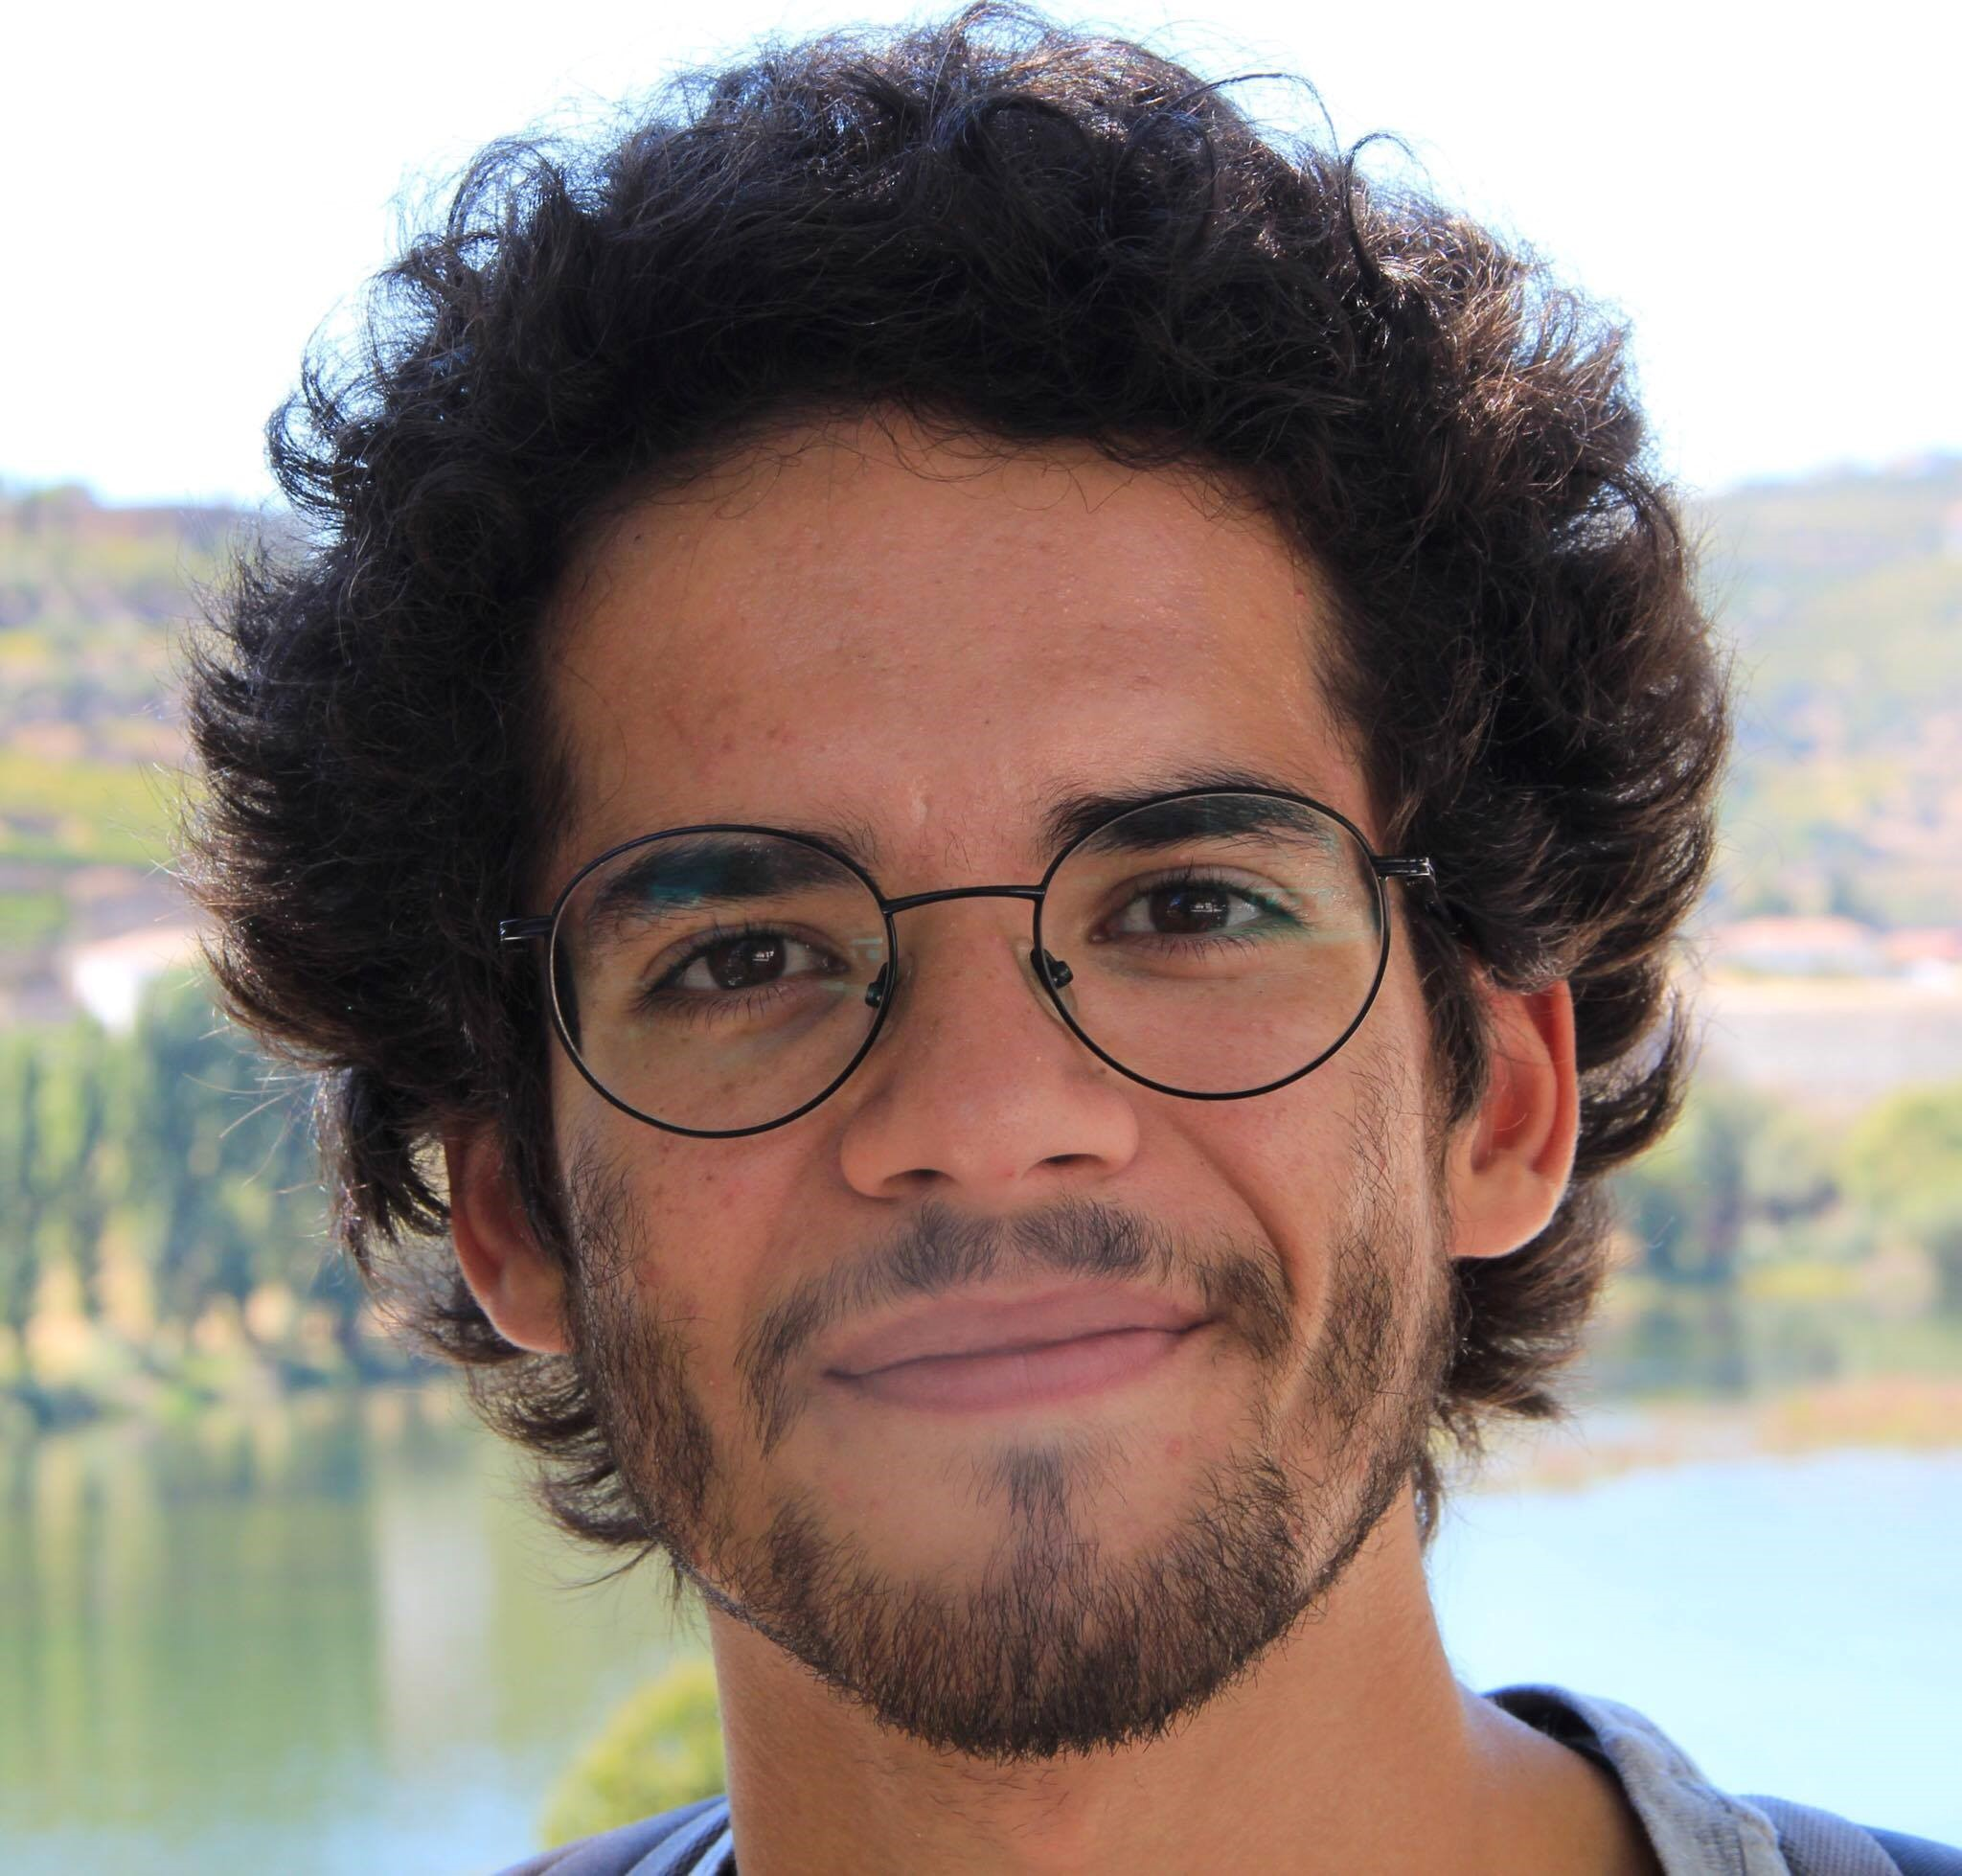
\includegraphics[width=1.5cm]{afonso.jpg}\break
    Marco Silva\textsc{(A79607)}\\
    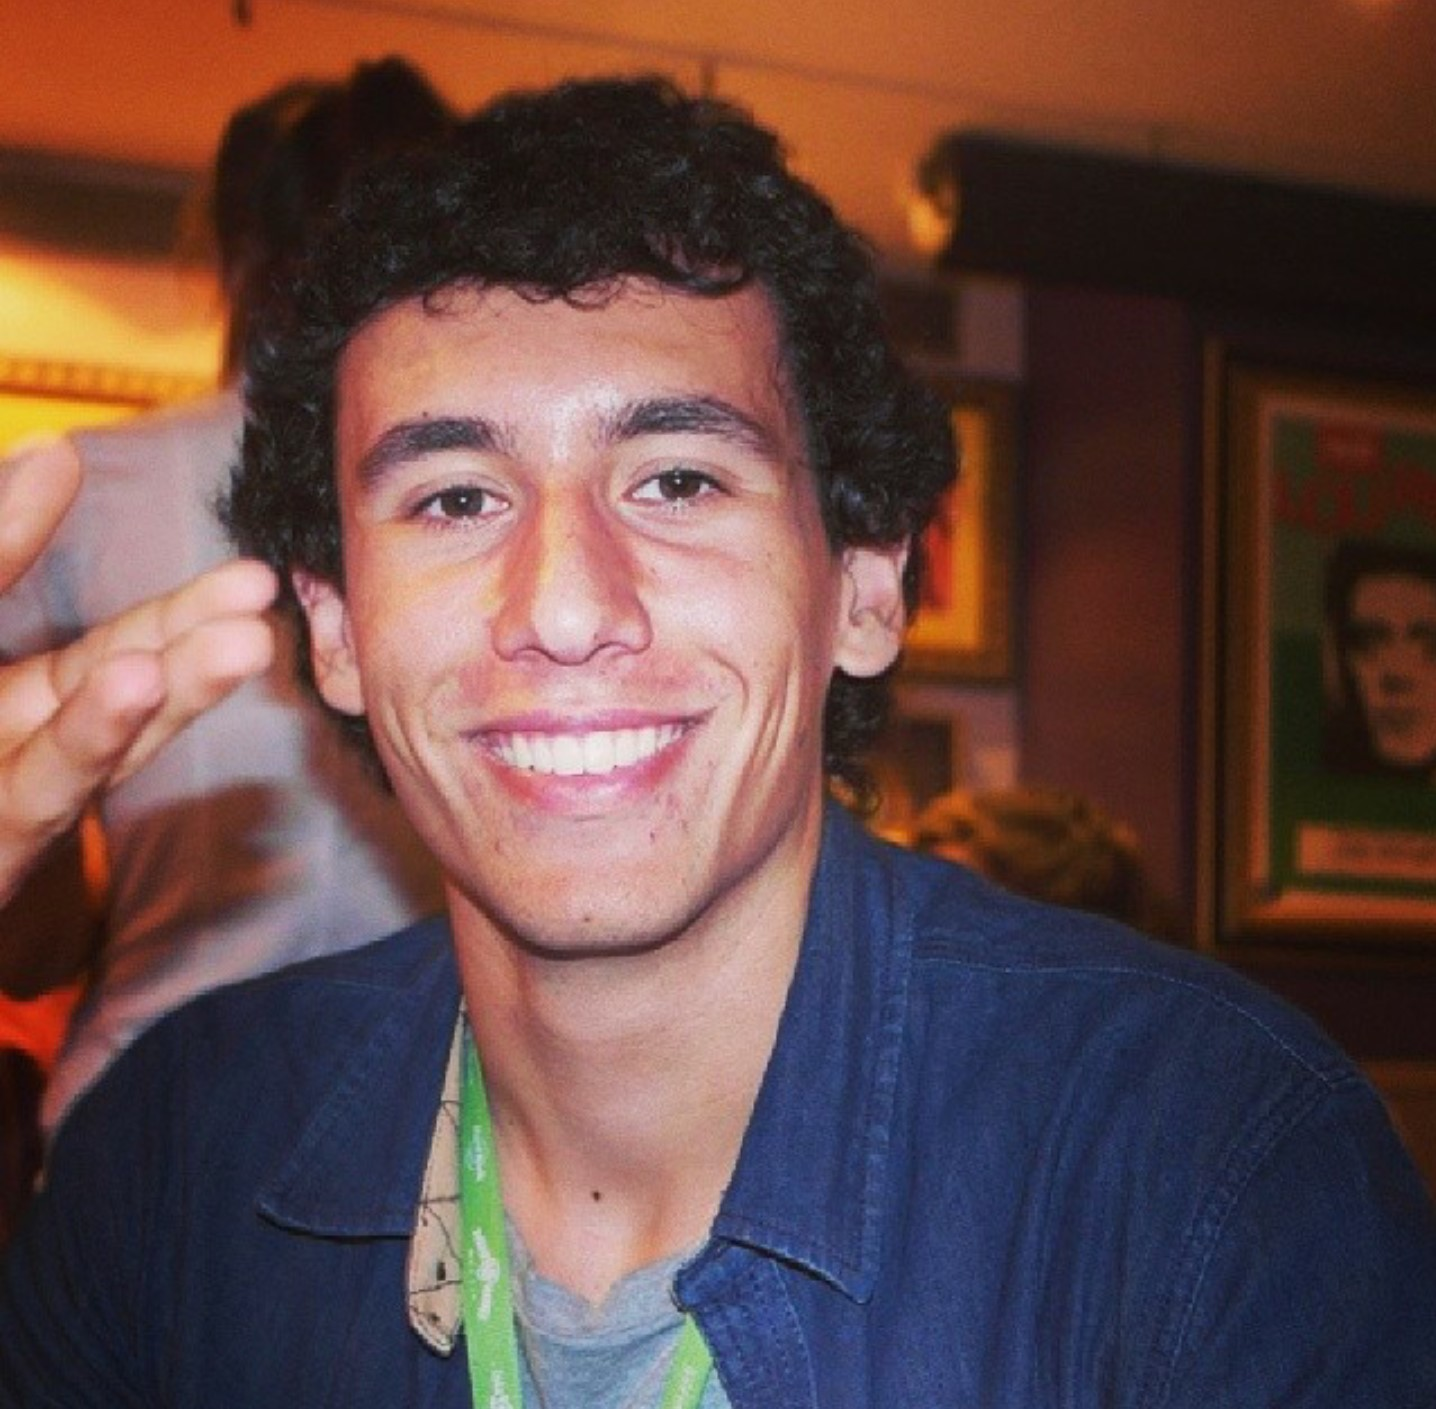
\includegraphics[width=1.5cm]{marco.jpg}\break
  \end{flushleft}
\end{minipage}%
\vfill

% Bottom of the page
{\large Versão 1.0 \\ \today}

\end{center}
\end{titlepage}


\begin{abstract}%DANIEL

\hspace{3mm} O objetivo desta fase do trabalho prático é criar cenas hierárquicas em XML recorrendo a transformações geométricas. Uma cena é definida por uma árvore cujos nodos contêm um conjunto de transformações geométricas, nomeadamente, \textit{translate, rotate} e \textit{scale}, e, opcionalmente, um conjunto de modelos. Cada poderá ter também um ou mais filhos. 

\par Para demonstrar o resultado do trabalho nesta fase, definir-se-á também uma cena com o modelo estático do sistema solar, com o Sol, os planetas e luas, definidos numa hierarquia.

\end{abstract}

\pagebreak
\tableofcontents

\pagebreak

% ===================================================
\section{Introdução}%DANIEL

\hspace{3mm} Tendo na fase anterior sido construídas uma aplicação \textit{generator}, que cria modelos primitivos de figuras, e uma aplicação \textit{engine}, capaz de demonstrar as figuras referidas através de um ficheiro de configuração em XML, proceder-se-á ao desenvolvimento de funcionalidades do \textit{engine}. Inicialmente, este teve apenas a capacidade de desenhar primitivas no ecrã exatamente como foram definidas pelo \textit{generator}. Como se pretende utilizar este programa para renderizar cenas, será necessário que este consiga efetuar \textbf{transformações geométricas}.

\par Uma transformação geométrica define-se como uma função que altera as propriedades de um ou mais eixos de coordenadas, geralmente em $\mathbb{R}^2$ ou $\mathbb{R}^3$. Através destas, é possível desenhar figuras mais complexas a partir de primitivas simples. Para este projeto, focou-se especificamente em três:  

\begin{itemize}
    \item Translações, que movem a origem do sistema de coordenadas por um vetor de coordenadas \texttt{(u,v,w)};
    \item Rotações, que rodam um ou mais eixos de coordenadas no sentido anti-horário à volta de um ângulo $\alpha$;
    \item Escalas, que aumentam ou diminuem a distância entre unidades de comprimento de um ou mais eixos do sistema de coordenadas.
\end{itemize}

\par Uma \textbf{cena} define-se como uma árvore cujos nodos contêm um conjunto das transformações geométricas descritas, bem como, opcionalmente, um conjunto de modelos primitivos e um grupo de nodos filho. Qualquer nodo filho herdará as transformações aplicadas ao respetivo pai. Transformações geométricas existem exclusivamente dentro de um grupo e são aplicadas a todos os modelos e subgrupos.

\par Tendo atualizado as capacidades do \textit{engine}, proceder-se-á ao desenvolvimento de um ficheiro XML que descreva um modelo do nosso Sistema Solar para demonstrar o funcionamento do programa. É de notar que as primitivas utilizadas pelo ficheiro XML em questão serão criadas pela aplicação \textit{generator} existente.

% ===================================================
\section{Descrição do Trabalho e Análise de Resultados}

\subsection{Sistema solar em XML} 

\subsubsection{Estrutura do XML}

\hspace{3mm} A descrição do sistema solar será feita através de um ficheiro \emph{XML}. Este ficheiro, encontra-se estruturado sob a forma de uma árvore em que cada um dos seus nodos poderá conter um conjuntos de transformações e um ou mais modelos que devem ser representados. Estes são ficheiros .3d gerados pelo \emph{generator} que contêm a representação das formas a desenhar sobre a forma de pontos.

\par Teremos então como possibilidade nodos do tipo \emph{group} e \emph{models}. Tem-se ainda o nodo \emph{scene} que constituirá a árvore de representação de uma cena completa. Em qualquer um dos tipos de nodos podem também ser definidos novos nodos, também designados por nodos filhos. Todas as transformações definidas em nodos de nível acima na árvore do ficheiro deverão ter efeito em nodos de maior profundidade e consequentemente, o efeito de qualquer transformação não se deve propagar para grupos de profundidade inferior na árvore de representação da cena. Estas transformações apenas podem existir dentro de nodos do tipo \emph{group} e devem ser consideradas apenas dentro do mesmo. De salientar ainda que, a ordem pela qual as transformações são definidas terá de ser considerada no momento do desenho da cena.

\pagebreak
% Falar da pesquisa feita [DANIEL]
\subsubsection{O Sistema Solar}

\hspace{3mm} Neste ponto será descrito o modelo do Sistema Solar desenvolvido para demonstrar o resultado do trabalho nesta fase. Pretende-se que desenhar um modelo à escala que inclua o Sol\cite{sun}, os planetas (Mercúrio\cite{mercury}, Vénus\cite{venus}, Terra\cite{earth}, Marte\cite{mars}, Júpiter\cite{jupiter}, Saturno\cite{saturn}, Úrano\cite{uranus} e Neptuno\cite{neptune}, bem como o planeta anão Plutão\cite{pluto}) e a Lua\cite{moon}. Como referência, utilizou-se o raio da Terra, $rT = 6371.0 km$, para efetuar os cálculos necessários, que no \textit{OpenGL} serão utilizados num rácio de conversão de $1 rT = 0.5 u.c$ (unidades de comprimento) para determinar as dimensões de cada objeto (com a exceção do Sol). 

\par Como seria de esperar, todos os corpos celestes aqui descritos serão esferas. Excecionalmente, Saturno apresentará os seus anéis\cite{sat_rings}, representados como um único no modelo em questão, cujos raios interior e exterior são 1.5 u.c e 2.0 u.c, respetivamente.

\par Primeiramente, o Sol, é um corpo com um raio de $109 rt$, centrado na origem do referencial. No entanto, como isto tornaria os restantes corpos celestes minúsculos - praticamente invisíveis - por comparação, por motivos práticos, o seu raio será imposto a $20 u.c$ no \textit{OpenGL}.

\par Seguindo as guias descritas anteriormente, os planetas terão os seguintes raios:
\begin{itemize}
    \item Mercúrio: 0.1915 u.c;
    \item Vénus: 0.4750 u.c;
    \item Terra: 0.5000 u.c . Adicionalmente, a Lua terá um raio de 0.1000 u.c;
    \item Marte: 0.2665 u.c;
    \item Júpiter 5.6045 u.c;
    \item Saturno: 4.7245 u.c;
    \item Úrano: 2.000 u.c;
    \item Neptuno: 1.9400 u.c;
    \item Plutão: 0.0900 u.c;
\end{itemize}

\par Quanto às órbitas de cada planeta e da Lua, devido à sua disparidade, decidiu-se impor que Plutão orbitará o Sol a $530 u.c$, com os restantes corpos distando uns dos outros proporcionalmente a esta distância. Sendo assim, cada planeta orbitará o Sol às seguintes distâncias:
\begin{itemize}
    \item Mercúrio: 34.9025 u.c;
    \item Vénus: 39.1599 u.c;
    \item Terra: 42.6646 u.c . Adicionalmente, a Lua orbitará a Terra a 3.000 u.c de distância;
    \item Marte: 49.2969 u.c;
    \item Júpiter 95.9121 u.c;
    \item Saturno: 151.3596 u.c;
    \item Úrano: 273.3941 u.c;
    \item Neptuno: 410.9605 u.c;
    \item Plutão: 530.0000 u.c;
\end{itemize}

\subsubsection{Hierarquia do Sistema Solar}

\hspace{3mm} Tendo em conta a estruturação do ficheiro \emph{XML} definida mais a cima neste relatório, o sistema solar encontra-se representado em apenas uma cena, constituída por vários grupos.

\par Para que a interpretação do ficheiro de representação do sistema solar fosse o mais direta possível, os elementos constituintes do mesmo foram definidos começando no centro pelo Sol e, finalmente, os restantes planetas e respetivas luas, começando pelos com menor raio de órbita e terminando nos mais longínquos.

\par Para cada um dos planetas, foi então definido um nodo do tipo \emph{group} que contem todas as primitivas essenciais para uma correta representação do mesmo. Este isolamento é essencial para que as transformações não tenham efeito na restante cena.

\par Deste modo, para cada um dos planetas, para além do seu desenho, foi também representada a sua órbita através da adição de uma nova opção de desenho no \emph{generator}.

\begin{lstlisting}[language=C++, caption=Algoritmo utilizado para a geração de uma órbita.]
    vector <Point> orbit_generate_points(vector <Point> points, float radius){

        Point p;

        int sides = 1000;
        float increment = (2*M_PI) / sides;

        for (int i = 0; i  < sides; i += 2){

            p.setPoint(radius * sin(increment * i), 0, radius * cos(increment * i));
            points.push_back(p);
            p.setPoint(radius * sin(increment * (i + 1)), 0, radius * cos(increment * (i + 1)));
            points.push_back(p);
            p.setPoint(radius * sin(increment * (i + 1)), 0, radius * cos(increment * (i + 2)));
            points.push_back(p);

        }

        return points;
    }
\end{lstlisting}

\par Tendo em conta o código acima apresentado, para a geração de uma representação da trajetória do planeta, o mais óbvio seria a geração de pares de pontos tendo em conta um determinado incremento no ângulo.

\par Quando observado o método de desenho no \emph{engine}, nota-se que a maioria das figuras é desenhada com base em triângulos, exigindo a opção \emph{GL\_TRIANGLES}, como podemos ver acima. De modo a manter esta característica, é fornecido um ponto extra ao necessário, para que seja possível representar linhas sem a opção \emph{GL\_LINE}.

\par Estando a órbita representada, será agora necessário representar o planeta e as suas luas. Para isso, foi definido um novo grupo, uma vez que a orbita é desenhada a partir do centro do sistema solar mas o planeta e todos os seus componentes terão de sofrer uma translação.

\par Vejamos agora o caso particular do desenho do planeta Terra, Lua e respetiva órbita. Numa primeira fase, ainda com o referencial centrado na origem do sistema solar, procede-se ao desenho da órbita da Terra. Para isso, recorre-se ao ficheiro \textit{orbit.3d} que contém a descrição de uma órbita de raio 1. Para que esta seja desenhada com o raio correto, aplica-se um \emph{scale} com o valor do raio pretendido. Esta operação terá de estar contida num nodo, uma vez que de seguida pretendemos partir novamente da origem do sistema solar. Após o desenho da órbita, efetua-se um \emph{translate} no eixo do X por forma a que, quando a esfera for desenhada, coincida com a orbita anteriormente descrita. Deste modo, temos assim representado o planeta Terra e a sua órbita.
\par Para o desenho da Lua e respetiva órbita, o raciocínio adotado é análogo, tendo apenas em consideração que o ponto de partida não será o centro do sistema solar mas sim o centro do planeta Terra, estando estes num grupo conjunto.

\begin{lstlisting}[language=XML, caption=Representação de um exemplo de criação de nodos filhos.]
    <!-- TERRA -->
        <!-- desenho da orbita da terra -->
        <group>
            <scale X="42.66465321" Y="42.66465321" Z="42.66465321"/>
            <models>
                <model file="orbit.3d"/>
            </models>
        </group>
        <!-- desenho do conjunto: Terra, Lua e respetiva orbita -->
        <group>
            <translate X="42.66465321" Y="0" Z="0"/>

            <scale X="0.5" Y="0.5" Z="0.5"/>
            <models>
                <model file="sphere.3d"/>
            </models>

            <!-- desenho da orbita da Lua -->
            <group>
                <scale X="3" Y="3" Z="3"/>
                <models>
                    <model file="orbit.3d"/>
                </models>
            </group>

            <!-- desenho da Lua -->
            <group>
                <translate X="3" Y="0" Z="0"/>
                <scale X="0.1" Y="0.1" Z="0.1"/>
                <models>
                    <model file="sphere.3d"/>
                </models>
            </group>

        </group>
\end{lstlisting}

\par Desta forma, são feitas as transformações necessárias à representação correta do planeta Terra, da Lua e respetiva orbita. Devido à estrutura em árvore, as transformações para a representação da Lua não têm efeito nas restantes representações.



% ---------------------------------------------------

\subsection{Carregamento do XML} %[AFONSO]

\hspace{3mm} O \textit{engine} é um componente responsável por concretizar efetivamente a cena. No entanto, fá-lo com completa abstração quanto àquilo que está a desenhar. Desta forma, é o próprio ficheiro XML passado por argumento ao \textit{engine} que é responsável por organizar a cena e estruturar todas as suas primitivas de forma a produzir o resultado desejável.

Assim sendo, é necessário carregar o conteúdo do ficheiro XML havendo para o efeito duas abordagens possíveis, fazer \textit{parse} deste documento todas as vezes que fosse necessário redesenhar a cena ou apenas fazer \textit{parse} do ficheiro uma vez, carregar os dados para uma estrutura de dados e redesenhar a cena com base nesta. A abordagem escolhida foi a segunda visto que o acesso a ficheiros é inevitavelmente uma operação muito custosa que iria ser repetida um número elevadíssimo de vezes. Assim, o \textit{parse} do ficheiro é apenas realizado uma vez e, posteriormente, quando for necessário o acesso à informação da cena, este é realizado diretamente à estrutura de dados criada para o efeito. No caso concreto deste projeto, o carregamento do XML é realizado através da biblioteca \textit{Pugixml} \cite{pugixml}.

\begin{figure}[h]
    \centering
    \begin{subfigure}{0.5\textwidth}
        \centering
        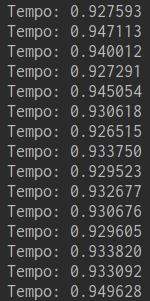
\includegraphics[width=0.5\linewidth]{tempos_bef_upgrade.png}
        \caption{Tempos de execução fazendo parse do ficheiro XML.}
    \end{subfigure}%
    \begin{subfigure}{0.5\textwidth}
        \centering
        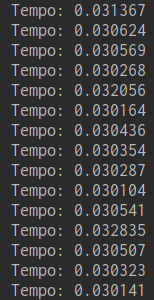
\includegraphics[width=0.5\linewidth]{tempos_pos_upgrade.png}
        \caption{Tempos de execução percorrendo a estrutura de dados \texttt{Group}.}
    \end{subfigure}
    \label{fig:tempos}
\end{figure}

\newpage

Os tempos foram obtidos através do cálculo da diferença entre o \texttt{timestamp} antes da execução da função \texttt{parseXML}, no caso da leitura direta do ficheiro e da função \texttt{drawGroup}. Além disso foi utilizado o mesmo ficheiro XML e mesma máquina para produzir a comparação mais fiel possível.

\begin{lstlisting}[language=C++, caption=Função usada na obtenção dos tempos de execução.]
    #include <sys/time.h>
    typedef unsigned long long timestamp_t;

    static timestamp_t get_timestamp ()
    {
      struct timeval now;
      gettimeofday (&now, NULL);
      return  now.tv_usec + (timestamp_t)now.tv_sec * 1000000;
    }

    void renderScene() {
        ...
        timestamp_t t0 = get_timestamp();
        
        parseXML(); 
            OU 
        scene.drawGroup();
        
        timestamp_t t1 = get_timestamp();
    
        double secs = (t1 - t0) / 1000000.0L;
        
        printf("Tempo: %lf\n", secs);
        ...
    }
\end{lstlisting}


Deste modo, foi criada uma estrutura de dados capaz de armazenar os dados presentes no ficheiro XML. Esta teria de conter um \texttt{group}, que por sua vez conteria um \texttt{translate}, \texttt{rotate}, \texttt{scale}, \texttt{models}, e novamente um \texttt{group}. Ainda, o elemento \texttt{models} pode conter um ou mais \texttt{model}. Todos este componentes são no entanto opcionais e como tal nem todos precisam de estar sempre presentes. De forma a auxiliar a representação do um ponto genérico, ou seja, constituído por uma coordenada x, y e z, foi criada uma classe Point que representa exatamente esse modelo de dados. Assim sendo, dentro da classe \texttt{Group} existe um \texttt{Point translate}, que armazena as coordenadas necessárias à realização \textit{translate}, existe um \texttt{float angle} que juntamente com um \texttt{Point rotate} permitem executar rotações aos modelos do grupo em questão, existe um \texttt{vector<Model> models} que permite armazenar todos os modelos presente neste elemento, a classe \texttt{Model} por sua vez representa todos os pontos da primitiva expressa em cada um dos ficheiros 3d e como tal apenas tem como variável um \texttt{vector<Point> primitive}, ou seja, um vetor com todos os pontos necessários para desenhar determinada figura. Por fim, a classe \texttt{Group} contém um \texttt{vector<Group *> groups} que fica responsável por agrupar num vetor com os apontadores para todos os grupos que um determinado grupo possa integrar, surgindo desta forma recursividade no tipo de dados. 

\begin{figure}[h]
    \centering
    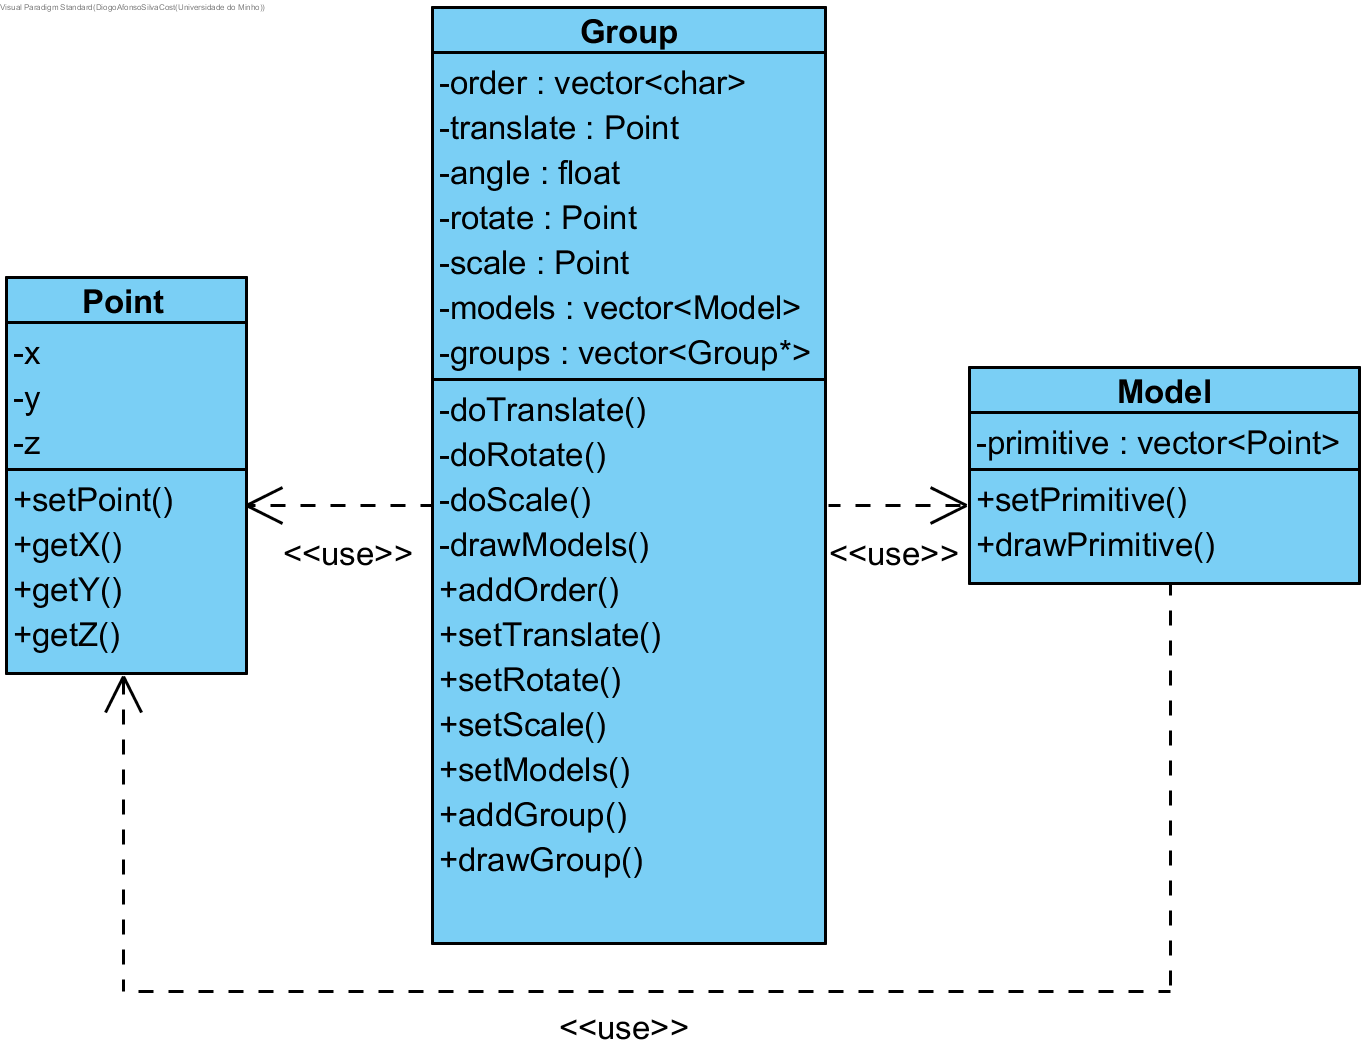
\includegraphics[width=0.7\linewidth]{Scene.png}
    \caption{Estrutura de dados utilizada.}
    \label{fig:classses}
\end{figure}

O \textit{parse} do ficheiro XML propriamente dito é realizado com base em iteradores disponíveis na biblioteca \textit{Pugixml}. Primeiramente, é encontrado o elemento \textit{"scene"}.

\begin{lstlisting}[language=C++, caption=Elemento \textit{scene}.]
    pugi::xml_node groups = doc.child("scene");
\end{lstlisting}

Cada um dos seus eventuais nodos é visitado através de um iterador. Caso algum destes seja um \texttt{group}, este é processado e o resultado é adicionado à variável \texttt{groupDest} que será, consequentemente, a variável global da estrutura de dados \texttt{scene}.

\begin{lstlisting}[language=C++, caption=Adição de um novo nodo \texttt{group}.]
    Group * groupDest = new Group();

    for (pugi::xml_node_iterator it = groups.begin(); it != groups.end(); ++it) {
        if (strcmp(it->name(), "group") == 0) {
            (*groupDest).addGroup(parseGroup(it)); 
        }
    }

    scene = *groupDest;
\end{lstlisting}

O processamento do nodo \texttt{group} é certamente o ponto fulcral do \textit{parsing} do XML. Deforma a percorrer todas as estruturas adjacentes a um determinado \texttt{group} é repetido o método referenciado anteriormente, ou seja, é criado um iterador. De seguida, é dado um tratamento diferenciado caso o elemento que surge numa iteração em específico, isto é, caso seja um \texttt{translate}, \texttt{rotate}, \texttt{scale}, \texttt{models}, ou novamente um \texttt{group}. No caso do \texttt{translate} é chamada a função \texttt{parseTranslate}. Esta função percorre, com a ajuda de um iterador, todos os atributos do elemento \texttt{translate} e com a ajuda da função \texttt{strtof} converte os valores de x, y e z de string para \texttt{float} para que sejam devidamente armazenados na variável \texttt{Point translate} presente na classe \texttt{Group}. No entanto, é importante referir que não é obrigatório que apareçam as três coordenadas no ficheiro XML e como tal por omissão essas coordenadas ficam com o valor 0.

\begin{lstlisting}[language=C++, caption=\textit{Parse} do nodo \texttt{translate} e consequente carregamento para a estrutura de dados.]
    Point parseTranslate(pugi::xml_node_iterator translate) {

        Point p; float x = 0, y = 0, z = 0;

        for (pugi::xml_attribute_iterator ait = translate->attributes_begin(); ait != translate->attributes_end(); ++ait)
        {
            if (strcmp(ait->name(), "X") == 0) {
                x = strtof(ait->value(), nullptr);
            }
            ...
        }

        p.setPoint(x,y,z);
        return p;
    }


    Group* parseGroup(pugi::xml_node_iterator groupSrc) {
        ...
        if (strcmp(it->name(), "translate") == 0) {
                (*groupDest).setTranslate(parseTranslate(it));
                (*groupDest).addOrder('t');
        }
        ...
    }
\end{lstlisting}

De forma análoga, o processo repete-se para as premissas \texttt{rotate} e \texttt{scale}. Além disso, como é possível constatar na porção do código da função \texttt{parseGroup} existe um carácter "t" que é adicionada a uma variável na classe \texttt{Group}. A variável em questão é um \texttt{vector<char> order} que está responsável por manter a ordem pela qual o \texttt{translate}, o \texttt{rotate} e o \texttt{scale} aparecem no ficheiro XML, visto que a sua alteração induz em diferentes cenas finais. No caso do \texttt{translate} é adicionado um "t", no \texttt{rotate} é adicionado um "r" e para o \texttt{scale} um "s".

No caso do \texttt{models} é chamada a função \texttt{parseModels}. Esta função realiza o \textit{parse}, com a ajuda de um iterador, de todos os componentes \textit{model} através do \texttt{parseModel}. Por sua vez, o \texttt{parseModel} extrai o nome do ficheiro presente no atributo \textit{file} e passa-o à função \texttt{loadModel}. Por fim esta percorre o ficheiro de um determinada primitiva, converte as coordenadas nele presentes de \texttt{string} para \texttt{float} através da função \texttt{strtof} \cite{strtof}, agrupa as coordenadas de três em três para formar um ponto concreto, constrói uma variável \texttt{Point} com eles e, por fim, adiciona o ponto ao \texttt{vector} da classe \texttt{Model}.

\begin{lstlisting}[language=C++, caption=\textit{Parse} do nodo \texttt{models} e consequente carregamento para a estrutura de dados.]
    void loadModel(const pugi::char_t *string, Model* model) {

        vector<Point> primitive;
        
        ...
        
        while (getline(fs, buffer)) {

            vector<std::string> aux;
            split(buffer, ' ', aux);
            buffer_points[i * 3 + 0] = strtof(aux[0].c_str(),0);
            buffer_points[i * 3 + 1] = strtof(aux[1].c_str(),0);
            buffer_points[i * 3 + 2] = strtof(aux[2].c_str(),0);

            i++;

            if (i == 3) {

                p.setPoint(buffer_points[0], buffer_points[1], buffer_points[2]);
                primitive.push_back(p);
                p.setPoint(buffer_points[3], buffer_points[4], buffer_points[5]);
                primitive.push_back(p);
                p.setPoint(buffer_points[6], buffer_points[7], buffer_points[8]);
                primitive.push_back(p);

                i = 0;
            }

        }
        
        ...

        (*model).setPrimitive(primitive);
    }
\end{lstlisting}

Por último, no caso do \texttt{group} é chamada recursivamente a função \texttt{parseGroup}. O resultado é colocado no \texttt{vector<Group *> groups} na variável local \texttt{Group} e a variável local é devolvida após o processamento do \texttt{group} em questão.

\begin{lstlisting}[language=C++, caption=\textit{Parse} do nodo \texttt{group} e consequente carregamento para a estrutura de dados.]
    Group* parseGroup(pugi::xml_node_iterator groupSrc) {

        Group * groupDest = new Group();

        for (pugi::xml_node_iterator it = groupSrc->begin(); it != groupSrc->end(); ++it) {

            ...

            else if (strcmp(it->name(), "group") == 0) {
                (*groupDest).addGroup(parseGroup(it));
            }
        }

        return groupDest;
    }
\end{lstlisting}

Todo este processamento responsável pelo \textit{parsing} do ficheiro XML é apenas realizado um única vez na função \texttt{main} evitando desta forma que seja realizado múltiplas vezes ou mesmo aquando da execução da própria renderização da cena. Desta computação surge uma estrutura de dados pronta a ser acedida de forma eficiente e que permite produzir a cena presente no XML.



% ---------------------------------------------------

\subsection{Construção da cena} %[AFONSO]

\hspace{3mm} Após a estruturação do XML, o carregamento da informação deste para uma estrutura de dados, resta apenas desenhar a cena. Esta funcionalidade encontra-se integrada na função \texttt{drawGroup}, implementada na classe \texttt{Group}.

Assim sendo, quando é necessário desenhar um \texttt{group} é preciso ter em conta que todas as alterações realizadas dentro deste apenas têm influência nesse mesmo espaço de atuação, isto é, um \texttt{translate} realizado num \texttt{group} não tem qualquer influência num outro qualquer \texttt{group} desde que este não se encontre dentro do primeiro. Nesse caso as mudanças são acumulativas. De forma, a emular este comportamento são usadas as diretivas \texttt{glPushMatrix} e \texttt{glPopMatrix}. A primeira é executada sempre que se começa a processar um novo \texttt{group} e permite guardar numa \textit{stack} o referencial com as mudanças realizadas até ao momento. A segunda função é executada no final do desenho de um \texttt{group} por forma a restaurar o refetencial anteriormente guardado.

\begin{lstlisting}[language=C++, caption=Desenho das primitivas.]
    void Group::drawGroup() {
        glPushMatrix();
        ...
        glPopMatrix();
    }
\end{lstlisting}

Primeiramente, é necessário perceber qual a ordem pela qual o \texttt{translate}, \texttt{rotate} e o \texttt{scale} precisam de executados. Deste modo, é percorrido o vetor \texttt{order} e consoante o carácter executa-se a operação em questão. 

\begin{lstlisting}[language=C++, caption=Preservação da ordem das diretivas.]
    for (auto &it : order) {
        if (it == 't')
            doTranslate();
        else if (it == 'r')
            doRotate();
        else if (it == 's')
            doScale();
    }
\end{lstlisting}

De seguida, procede-se para o desenho dos modelos propriamente ditos com a ajuda da função \texttt{drawModels}. Esta por sua vez percorre o vetor \texttt{models} e para cada modelo executa a função \texttt{drawPrimitive} presente na classe \texttt{Model}. Esta por fim, agrupa os pontos do vetor \texttt{primitive} em conjuntos de três de forma a usar a função \texttt{glVertex3f} que agrupada por sua vez em conjuntos de três permite desenhar os triângulos que originarão a primitiva em questão.


\begin{lstlisting}[language=C++, caption=Desenho dos modelos.]
    void Model::drawPrimitive() {

        int i = 0;
        float buffer_points[9];

        for (auto &it : primitive) {

            buffer_points[i * 3 + 0] = it.getX();
            buffer_points[i * 3 + 1] = it.getY();
            buffer_points[i * 3 + 2] = it.getZ();

            i++;

            if (i == 3) {

                glBegin(GL_TRIANGLES);
                glVertex3f(buffer_points[0], buffer_points[1], buffer_points[2]);
                glVertex3f(buffer_points[3], buffer_points[4], buffer_points[5]);
                glVertex3f(buffer_points[6], buffer_points[7], buffer_points[8]);
                glEnd();

                i = 0;
            }
        }
    }


    void Group::drawModels() {
        for (auto &it : models) {
            it.drawPrimitive();
        }
    }
\end{lstlisting}

Por fim, é necessário desenhar os diversos grupos que possam estar contidos no \texttt{group} que está a ser processado. Para tal é iterado o vetor \texttt{groups} e para cada instância é chamada recursivamente a função \texttt{drawGroup}.

\begin{lstlisting}[language=C++, caption=Desenho do \texttt{group}.]
    void Group::drawGroup() {
        glPushMatrix();

        ...

        for (auto &it : groups) {
            it->drawGroup();
        }

        glPopMatrix();
    }
\end{lstlisting}

Ainda assim, o \texttt{renderScene} não é executado constantemente. De forma a otimizar ao máximo o desempenho do \texttt{engine} foi utilizada a diretiva \texttt{glutPostRedisplay} para que a cena apenas fosse redesenhada quando houvesse alguma interação com o teclado ou rato que induzisse alguma alteração na composição da imagem.

\subsubsection{Resultado Final}

\hspace{3mm} Inicialmente, foi desenvolvida uma solução à escala real mas, devido à dimensão do sistema solar, não era clara a sua representação como um todo. Desta forma, foi desenvolvida uma segunda versão em que o principal foco seria aproximar a cena o mais possível da realidade sem nunca comprometer a visualização intuitiva do mesmo. Para que todo o sistema fosse visível dentro de uma só \emph{frame}, foram feitas algumas alterações nas escalas utilizadas para representar todo o sistema solar. Nomedamente, procedeu-se à redução do fator de escala do Sol de 109 rT para apenas 20 rT, e ainda à redução da distância real entre os planetas, mantendo sempre a proporção entre os mesmos.

\par Como resultado, é possível observar nesta nova solução o sistema solar.

\begin{figure}[h]
    \centering
    \begin{subfigure}{0.5\textwidth}
        \centering
        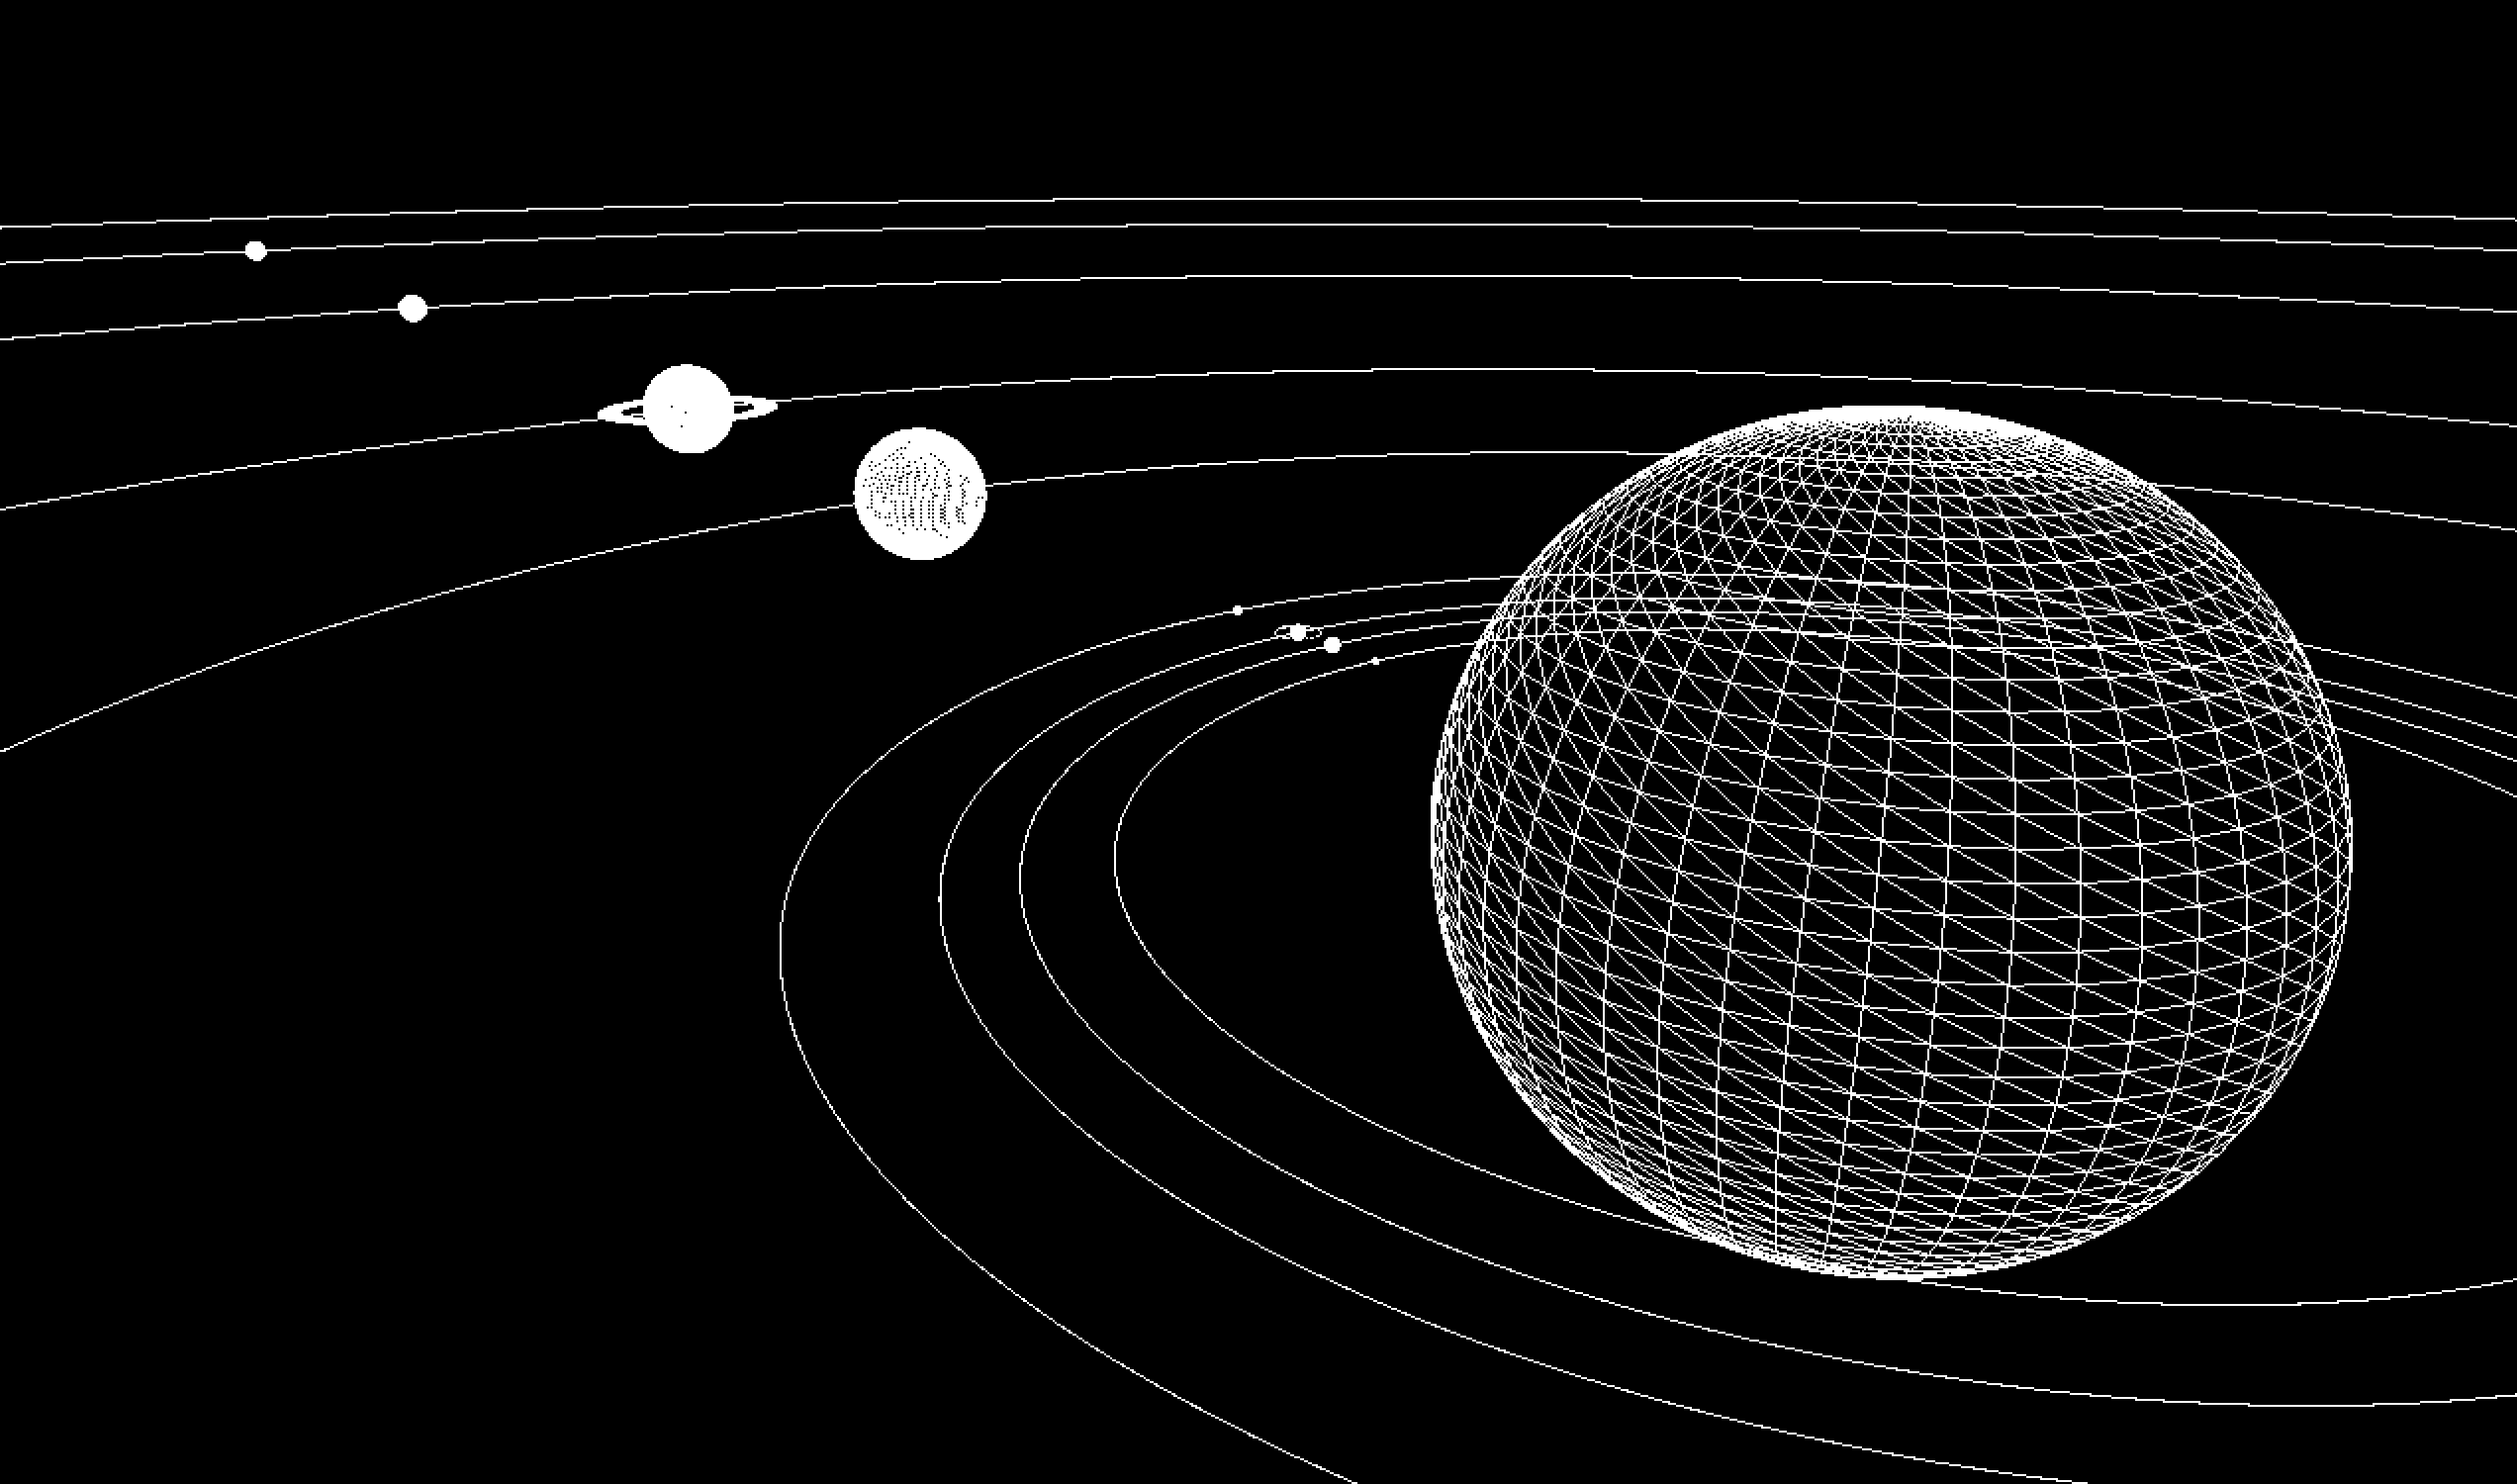
\includegraphics[width=0.95\linewidth]{solar_system_full.png}
        \caption{Demonstração completa do sistema solar.}
    \end{subfigure}%
    \begin{subfigure}{0.5\textwidth}
        \centering
        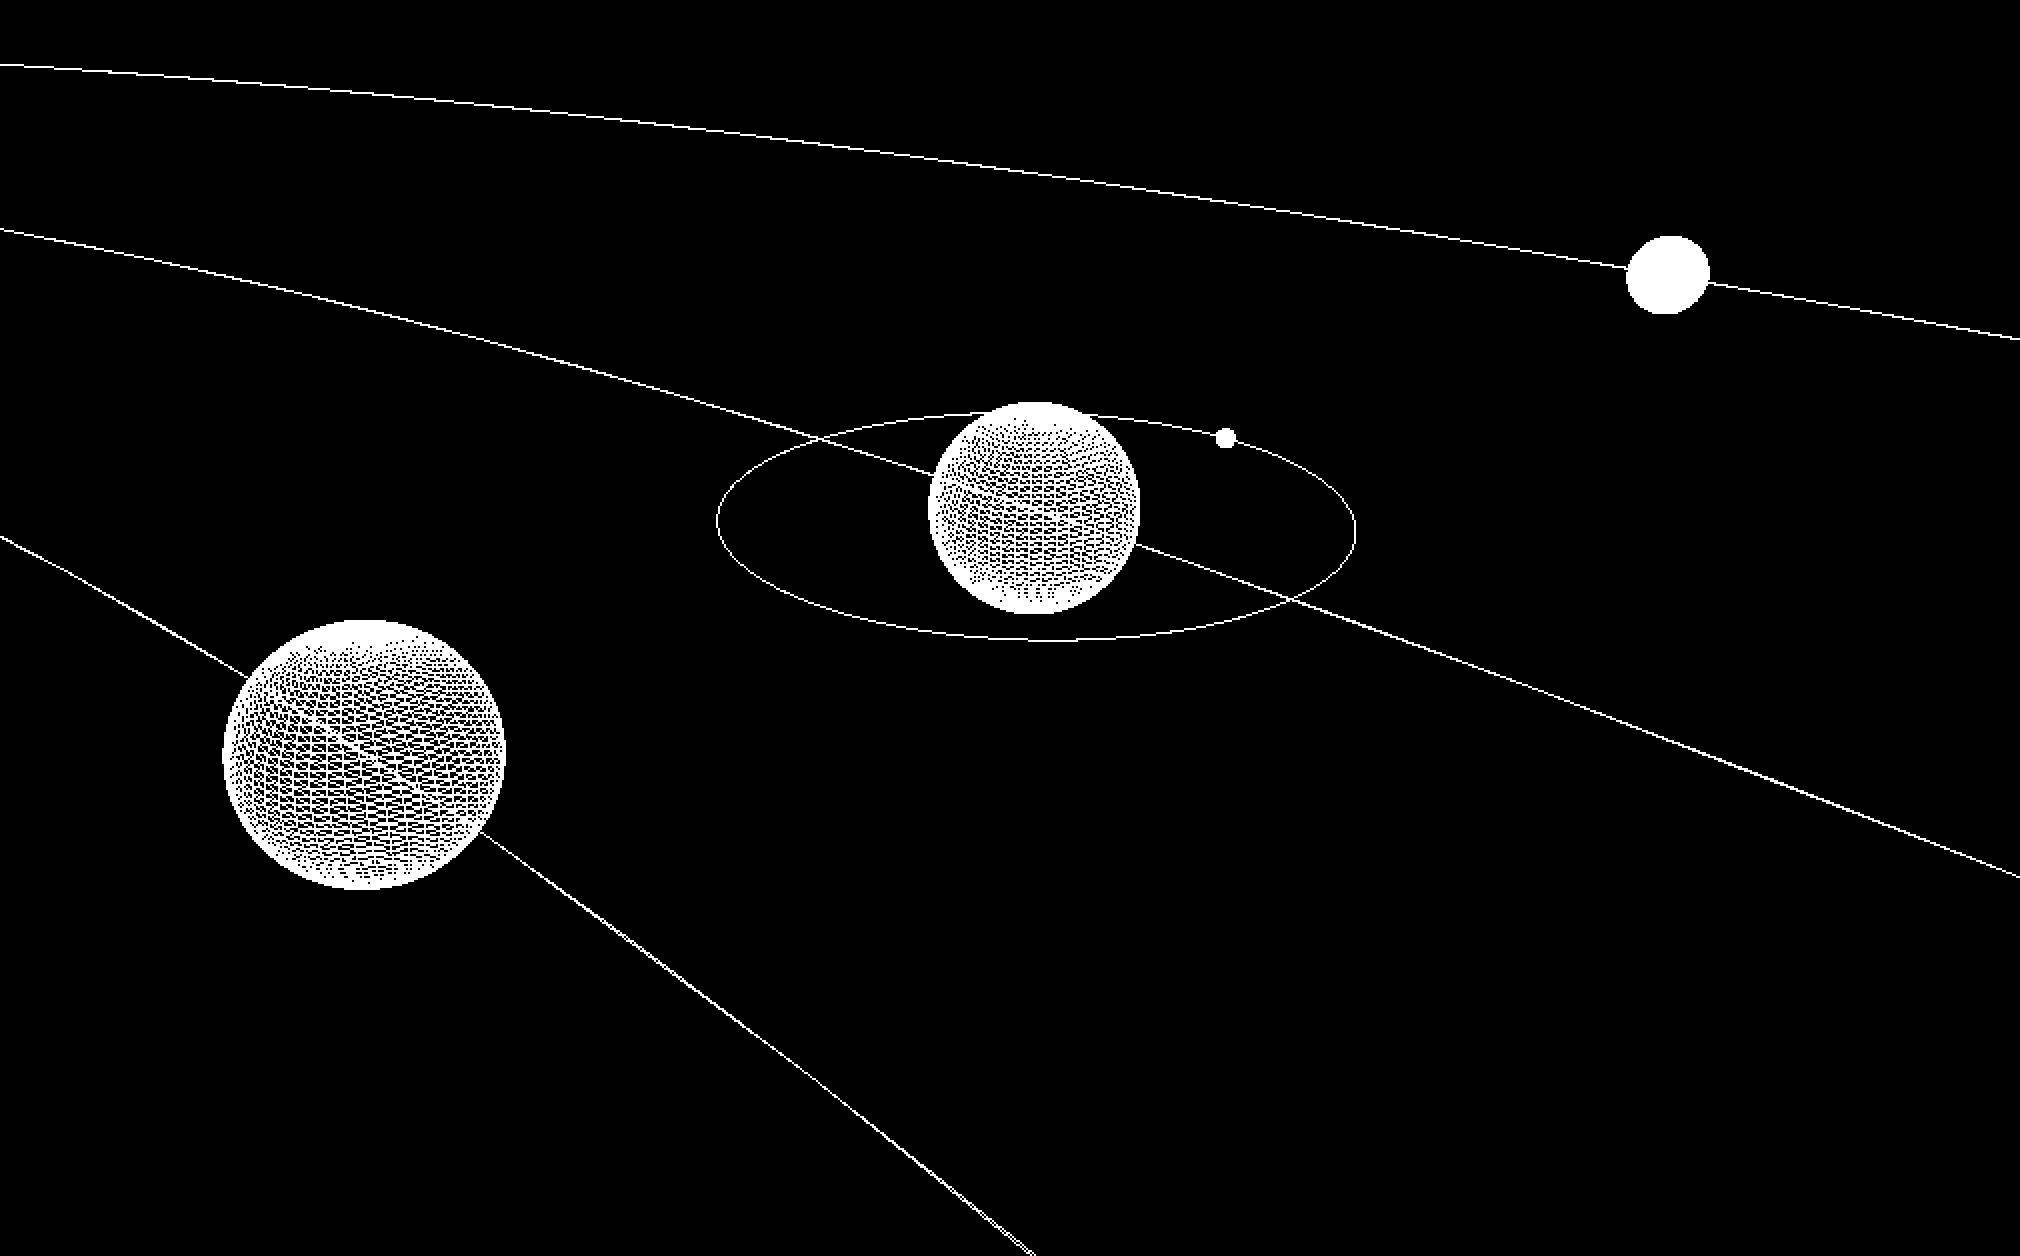
\includegraphics[width=0.95\linewidth]{solar_system_zoom1.png}
        \caption{Vista em pormenor dos planetas Vénus, Terra e respetiva Lua e finalmente Marte.}
    \end{subfigure}
    \label{fig:solar_system}
\end{figure}


\newpage
% ===================================================
\section{Conclusões e Sugestões}

\hspace{3mm} Nesta segunda fase do projeto, foram alcançadas as metas inicialmente definidas, mais concretamente, a representação de forma clara, elucidativa e eficiente do Sistema Solar. Com os dois modelos desenvolvidos, num deles é possível ter uma visão mais geral da constituição do mesmo enquanto que olhando para o sistema implementado à escala real, é-nos possível perceber a dimensão do nosso Sistema Solar.

\par Para além da representação visual, foi também notada uma especial importância relativamente à estruturação do documento \emph{XML}. Todos os requisitos apresentados por parte dos docentes facilitaram bastante no desenvolvimento da estrutura de dados mas também na implementação do \emph{parser}, facilitando assim a implementação das diversas transformações possíveis.

No entanto, existem alguns pormenores que podem e irão ser melhorados em fases seguintes do projeto, nomeadamente, a introdução de um nova primitiva o \texttt{torus}, que será utilizada para representar as diferentes órbitas e a adição de cor e textura aos diferentes componentes da cena.

Concluindo, é feito um balanço positivo no que toca ao trabalho desenvolvido nesta segunda fase do projeto, considerando que todas as dificuldades encontradas foram superadas, resultando um projeto coeso e modular.

\newpage
% ===================================================
\section{Anexos}

\begin{lstlisting}[language=XML]
    <scene>
    <group>
        <!-- SOL -->
        <group>
            <scale X="20" Y="20" Z="20"/>
            <models>
                <model file="sphere.3d"/>
            </models>
        </group>
        <!-- MERCURIO -->
        <group>
            <scale X="34.9025385" Y="34.9025385" Z="34.9025385"/>
            <models>
                <model file="orbit.3d"/>
            </models>
        </group>
        <group>
            <translate X="34.9025385" Y="0" Z="0"/>
            <scale X="0.1915" Y="0.1915" Z="0.1915"/>
            <models>
                <model file="sphere.3d"/>
            </models>
        </group>
        <!-- VENUS -->
        <group>
            <scale X="39.15998387" Y="39.15998387" Z="39.15998387"/>
            <models>
                <model file="orbit.3d"/>
            </models>
        </group>
        <group>
            <translate X="39.16066113" Y="0" Z="0"/>
            <scale X="0.47495" Y="0.47495" Z="0.47495"/>
            <models>
                <model file="sphere.3d"/>
            </models>
        </group>
        <!-- TERRA -->
        <group>
            <scale X="42.66465321" Y="42.66465321" Z="42.66465321"/>
            <models>
                <model file="orbit.3d"/>
            </models>
        </group>
        <group>
            <translate X="42.66465321" Y="0" Z="0"/>

            <scale X="0.5" Y="0.5" Z="0.5"/>
            <models>
                <model file="sphere.3d"/>
            </models>

            <group>
                <scale X="3" Y="3" Z="3"/>
                <models>
                    <model file="orbit.3d"/>
                </models>
            </group>

            <group>
                <translate X="3" Y="0" Z="0"/>
                <scale X="0.1" Y="0.1" Z="0.1"/>
                <models>
                    <model file="sphere.3d"/>
                </models>
            </group>

        </group>
        <!-- MARTE -->
        <group>
            <scale X="49.29685207" Y="49.29685207" Z="49.29685207"/>
            <models>
                <model file="orbit.3d"/>
            </models>
        </group>
        <group>
            <translate X="49.29685207" Y="0" Z="0"/>
            <scale X="0.2665" Y="0.2665" Z="0.2665"/>
            <models>
                <model file="sphere.3d"/>
            </models>
        </group>
        <!-- JUPITER -->
        <group>
            <scale X="95.91209462" Y="95.91209462" Z="95.91209462"/>
            <models>
                <model file="orbit.3d"/>
            </models>
        </group>
        <group>
            <translate X="95.91209462" Y="0" Z="0"/>
            <scale X="5.6045" Y="5.6045" Z="5.6045"/>
            <models>
                <model file="sphere.3d"/>
            </models>
        </group>
        <!-- SATURNO -->
        <group>
            <scale X="151.3596273" Y="151.3596273" Z="151.3596273"/>
            <models>
                <model file="orbit.3d"/>
            </models>
        </group>
        <group>
            <translate X="151.3596273" Y="0" Z="0"/>
            <scale X="4.7245" Y="4.7245" Z="4.7245"/>
            <models>
                <model file="sphere.3d"/>
                <model file="belt.3d"/>
            </models>
        </group>
        <!-- URANO -->
        <group>
            <scale X="273.3940626" Y="273.3940626" Z="273.3940626"/>
            <models>
                <model file="orbit.3d"/>
            </models>
        </group>
        <group>
            <translate X="273.3940626" Y="0" Z="0"/>
            <scale X="2" Y="2" Z="2"/>
            <models>
                <model file="sphere.3d"/>
            </models>
        </group>
        <!-- NEPTUNO -->
        <group>
            <scale X="410.960512" Y="410.960512" Z="410.960512"/>
            <models>
                <model file="orbit.3d"/>
            </models>
        </group>
        <group>
            <translate X="410.960512" Y="0" Z="0"/>
            <scale X="1.94" Y="1.94" Z="1.94"/>
            <models>
                <model file="sphere.3d"/>
            </models>
        </group>
        <!-- PLUTAO -->
        <group>
            <scale X="530" Y="530" Z="530"/>
            <models>
                <model file="orbit.3d"/>
            </models>
        </group>
        <group>
            <translate X="530" Y="0" Z="0"/>
            <scale X="0.09" Y="0.09" Z="0.09"/>
            <models>
                <model file="sphere.3d"/>
            </models>
        </group>
    </group>
</scene>

\end{lstlisting}

\newpage
% =========================================================
\bibliographystyle{unsrt}
\bibliography{biblio}


\end{document}